\section{Aufbau}
\label{sec:Aufbau}

Im Wesentlichen besteht die Apparatur aus dem optischen Teil, der Rubidiumprobe sowie der Messschaltung. Der komplette Aufbau
kann in Abbildung \ref{fig:aufbau} nachvollzogen werden.

\begin{figure}[H]
	\centering
	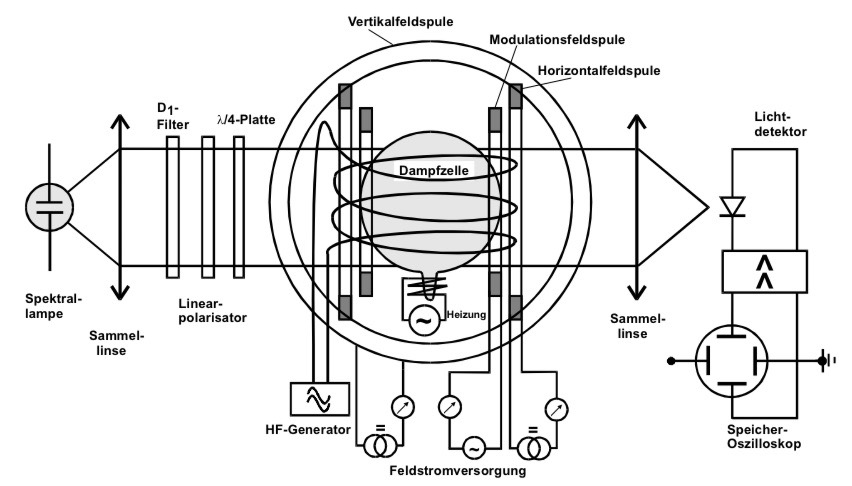
\includegraphics[width=0.8\linewidth]{content/grafik/aufbau.jpg}
	\caption{Schematische Aufsicht der gesamten Messapparatur. \cite{pumpen}}
	\label{fig:aufbau}
\end{figure}

Die Strahlungsquanten zur Anregung stammen aus einer Rubidiumspektrallampe, deren Licht zunächst durch eine Sammellinse kollimiert
und weiter mithile eines Interferenzfilters $D_1$ monochromatisiert wird. Um die erforderliche zirkulare Polarisation zu
erzeugen, wird ein $\lambda/4$ Plättchen verwendet, dem wiederum ein linearer Polarisationsfilter vorgeschaltet ist. Anschließend
durchdringt die Strahlung eine Rubidium Dampfzelle und pumpt die Besetzung wie zuvor beschrieben in erhöhte Zustände. Die
transmittierte Lichtintensität wird zuletzt auf einen Photodetektor fokussiert und das resultierende Signal in ein
Speicheroszilloskop gegeben. 

Um die Rubidiumprobe sind noch Helmholtz Spulenpaare angeordnet. Dabei erlaubt eine Vertikalfeldspule die Kompensation
der radialen Erdmagnetfeldkomponente. Mithilfe einer Modulationsfeldspule lässt sich dann ein Sweep über eine voreingestellte
Range an Magnetflussdichten in Kombination mit einer Radiofrequenzoszillation realisieren. Eine Horizontalfeldspule dient zur
Einstellung einer konstanten Verschiebung der Feldstärke bei Abbildung der Resonanzpeaks. 

Für die einzelnen Spulen gelten folgende Parameter:
\begin{align*}
	&& && && && &\text{Sweep: } & R &= \qty{16.39}{\centi\meter} & N &= \num{11} && && && && \\
	&& && && && &\text{Horizontal: } & R &= \qty{15.79}{\centi\meter} & N &= \num{154} && && && && \\
	&& && && && &\text{Vertikal: } & R &= \qty{11.735}{\centi\meter} & N &= \num{20} && && && &&
\end{align*}
